%\textit{•}%!TEX TS-program = xelatex

\documentclass[]{cv-class}
\usepackage{afterpage}
\usepackage{hyperref}
\usepackage{color}
\usepackage{xcolor}
\hypersetup{
    colorlinks=true,
    linkcolor=blue
}
\addbibresource{bibliography.bib}
\RequirePackage{xcolor}
\usepackage[utf8]{inputenc}
\usepackage[english]{babel} 
\usepackage[usenames, dvipsnames]{color}

\begin{document}

\begin{aside}
\color{blue}
%  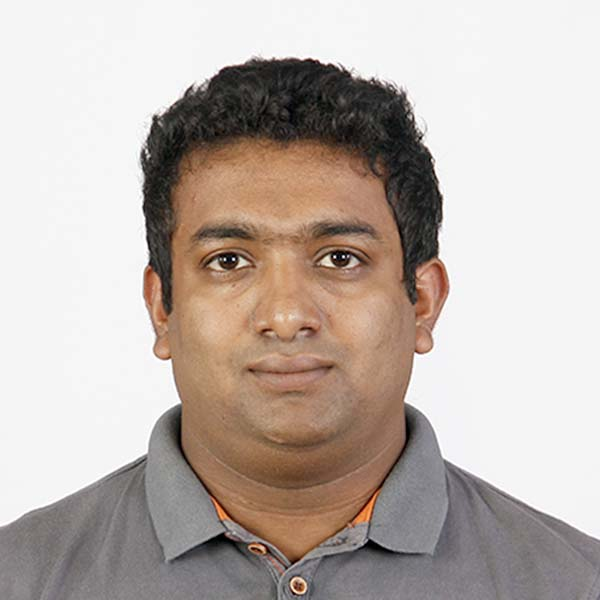
\includegraphics[scale=0.9]{img/photo.jpg}
%    ~
  \section{}
  	\vspace{0.5cm}
   ~  
  \header{Janitha}{Madushan}
      {Sr. Software Engineer}
   ~
%  \section{ADDRESS}
%    {\whitebodyfont No:04, "SunHill",\\
%    Vajirapura,\\
%    Nuwara-Eliya,\\
%    Sri-Lanka.}
%    ~
%  \section{MOBILE}
%    {\whitebodyfont +94 71 57 81 553\\
%    +94 75 97 46 502}
%    ~
  \section{MAILING}
    \underline{\href{mailto:janithasen@gmail.com}{{\whitebodyfont janithasen@gmail.com}}}
    ~
%  \section{LANGAUGES}
%  	{\whitebodyfont Sinhalese (Native)\\
%    Engilsh}
%    ~ 
%  \section{NIC}
%  	{\whitebodyfont 901540160V}
%    ~
%  \section{BIRTHDAY}
%  	{\whitebodyfont June 02,1990}
%    ~
  \section{WEB}
  	\vspace{0.10cm}
    \underline{\href{https://www.linkedin.com/in/janithamadushan}{{\whitebodyfont Linkedin}}}
    \\
	\vspace{0.10cm}
    \underline{\href{https://stackoverflow.com/users/4412223/janitha-madushan}{{\whitebodyfont Stackoverflow}}}
	\\	
	\vspace{0.10cm}
    \underline{\href{https://github.com/janitham}{{\whitebodyfont Github}}}
    ~
  \section{OS}
    \asidelist{{\whitebodyfont Windows}}
    {\includegraphics[scale=0.30]{img/star.png}
    \includegraphics[scale=0.30]{img/star.png}
    \includegraphics[scale=0.30]{img/star.png}
    \includegraphics[scale=0.30]{img/star.png}
    \includegraphics[scale=0.30]{img/star.png}}
    \asidelist{\whitebodyfont{Linux}}
    {\includegraphics[scale=0.30]{img/star.png}
    \includegraphics[scale=0.30]{img/star.png}
    \includegraphics[scale=0.30]{img/star.png}
    \includegraphics[scale=0.30]{img/star.png}
    \includegraphics[scale=0.30]{img/star_empty.png}}
    ~
  \section{LANGUAGES}
    \asidelist{{\whitebodyfont Java}}
    {\includegraphics[scale=0.30]{img/star.png}
    \includegraphics[scale=0.30]{img/star.png}
    \includegraphics[scale=0.30]{img/star.png}
    \includegraphics[scale=0.30]{img/star.png}
    \includegraphics[scale=0.30]{img/star.png}}
    \asidelist{\whitebodyfont{JavaScript}}
    {\includegraphics[scale=0.30]{img/star.png}
    \includegraphics[scale=0.30]{img/star.png}
    \includegraphics[scale=0.30]{img/star.png}
    \includegraphics[scale=0.30]{img/star.png}
    \includegraphics[scale=0.30]{img/star_empty.png}}
	\asidelist{\whitebodyfont{Pyhon}}
    {\includegraphics[scale=0.30]{img/star.png}
    \includegraphics[scale=0.30]{img/star.png}
    \includegraphics[scale=0.30]{img/star.png}
    \includegraphics[scale=0.30]{img/star.png}
    \includegraphics[scale=0.30]{img/star_empty.png}}
    \asidelist{\whitebodyfont{C}}
    {\includegraphics[scale=0.30]{img/star.png}
    \includegraphics[scale=0.30]{img/star.png}
    \includegraphics[scale=0.30]{img/star.png}
    \includegraphics[scale=0.30]{img/star.png}
    \includegraphics[scale=0.30]{img/star.png}}
    ~
  \section{TECHNOLOGIES}
    \asidelist{{\whitebodyfont Spring}}
    {\includegraphics[scale=0.30]{img/star.png}
    \includegraphics[scale=0.30]{img/star.png}
    \includegraphics[scale=0.30]{img/star.png}
    \includegraphics[scale=0.30]{img/star.png}
    \includegraphics[scale=0.30]{img/star.png}}
    \asidelist{\whitebodyfont{Hibernate}}
    {\includegraphics[scale=0.30]{img/star.png}
    \includegraphics[scale=0.30]{img/star.png}
    \includegraphics[scale=0.30]{img/star.png}
    \includegraphics[scale=0.30]{img/star.png}
    \includegraphics[scale=0.30]{img/star.png}}
    \asidelist{\whitebodyfont{Docker}}
    {\includegraphics[scale=0.30]{img/star.png}
    \includegraphics[scale=0.30]{img/star.png}
    \includegraphics[scale=0.30]{img/star.png}
    \includegraphics[scale=0.30]{img/star.png}
    \includegraphics[scale=0.30]{img/star_empty.png}}
	\asidelist{\whitebodyfont{Kubernetes}}
    {\includegraphics[scale=0.30]{img/star.png}
    \includegraphics[scale=0.30]{img/star.png}
    \includegraphics[scale=0.30]{img/star.png}
    \includegraphics[scale=0.30]{img/star.png}
    \includegraphics[scale=0.30]{img/star_empty.png}}    
    \asidelist{\whitebodyfont{Jenkins}}
    {\includegraphics[scale=0.30]{img/star.png}
    \includegraphics[scale=0.30]{img/star.png}
    \includegraphics[scale=0.30]{img/star.png}
    \includegraphics[scale=0.30]{img/star.png}
    \includegraphics[scale=0.30]{img/star.png}}
    \asidelist{\whitebodyfont{VSphere}}
    {\includegraphics[scale=0.30]{img/star.png}
    \includegraphics[scale=0.30]{img/star.png}
    \includegraphics[scale=0.30]{img/star.png}
    \includegraphics[scale=0.30]{img/star.png}
    \includegraphics[scale=0.30]{img/star_empty.png}}
    \asidelist{\whitebodyfont{AWS}}
    {\includegraphics[scale=0.30]{img/star.png}
    \includegraphics[scale=0.30]{img/star.png}
    \includegraphics[scale=0.30]{img/star.png}
    \includegraphics[scale=0.30]{img/star.png}
    \includegraphics[scale=0.30]{img/star_empty.png}}
    \asidelist{\whitebodyfont{GIT}}
    {\includegraphics[scale=0.30]{img/star.png}
    \includegraphics[scale=0.30]{img/star.png}
    \includegraphics[scale=0.30]{img/star.png}
    \includegraphics[scale=0.30]{img/star.png}
    \includegraphics[scale=0.30]{img/star_empty.png}}
    \asidelist{\whitebodyfont{Ansible}}
    {\includegraphics[scale=0.30]{img/star.png}
    \includegraphics[scale=0.30]{img/star.png}
    \includegraphics[scale=0.30]{img/star.png}
    \includegraphics[scale=0.30]{img/star_empty.png}
    \includegraphics[scale=0.30]{img/star_empty.png}}
    \asidelist{\whitebodyfont{Terraform}}
    {\includegraphics[scale=0.30]{img/star.png}
    \includegraphics[scale=0.30]{img/star.png}
    \includegraphics[scale=0.30]{img/star.png}
    \includegraphics[scale=0.30]{img/star_empty.png}
    \includegraphics[scale=0.30]{img/star_empty.png}}
    ~
      ~
  \section{DATABASES}
    \asidelist{{\whitebodyfont MySql}}
    {\includegraphics[scale=0.30]{img/star.png}
    \includegraphics[scale=0.30]{img/star.png}
    \includegraphics[scale=0.30]{img/star.png}
    \includegraphics[scale=0.30]{img/star.png}
    \includegraphics[scale=0.30]{img/star_empty.png}}
    \asidelist{\whitebodyfont{MsSql}}
    {\includegraphics[scale=0.30]{img/star.png}
    \includegraphics[scale=0.30]{img/star.png}
    \includegraphics[scale=0.30]{img/star.png}
    \includegraphics[scale=0.30]{img/star.png}
    \includegraphics[scale=0.30]{img/star_empty.png}}
	\asidelist{\whitebodyfont{Oracle}}
    {\includegraphics[scale=0.30]{img/star.png}
    \includegraphics[scale=0.30]{img/star.png}
    \includegraphics[scale=0.30]{img/star.png}
    \includegraphics[scale=0.30]{img/star_empty.png}
    \includegraphics[scale=0.30]{img/star_empty.png}}    
    ~
\end{aside}

\section{EDUCATION}
\begin{entrylist}
  \entry
    {Aug. 11 - June 15}
    {Computer Engineering}
    {Faculty of Engineering, University of Peradeniya, SriLanka}
    {   \\
        I have a BSc(Hons) degree which is specialized in “Computer Engineering”.
        In the university, I studied Electronics, Mathematics, Computer-Hardware \& Computer-Software as main parts of the course content.
    }
\end{entrylist}

\section{EXPERIENCE}
\begin{entrylist}
  \entry
    {Nov. 15 - Now}
    {Senior Software Engineer}
    {Cambio Software Engineering}
    {   \\
        Cambio Healthcare Systems is a Swedish based company that delivers products and services to the e-healthcare market over 20+ years.
        I have been working here for 4+ years as my first job opportunity \& currently working here as a “Senior Software Engineer”.
        \\
        \\
        “Cambio” has its own frameworks to implement the product based on Java.
        Therefore it has its own strategies/tools to Build, Release \& Deploy the product.
        I developed multiple tools/applications, have complex logic to support Build, Release \& Deployment phases, using cutting edge technologies.
        I have been working in an ‘Agile’ work environment.
        Also, I got the opportunity to work onsite in ‘Sweden’ \& work closely with the DevOps team as well.
        \\
        \\
        My strength is, I could convert any complex logic to the code.
    }
\\
  \entry
    {Oct. 15 - Mar.16}
    {Internship}
    {IFS R\&D}
    {   \\
        I involved in a R\&D project to expose their database entities as Restful resources.
        \textbf{ASP.NET, ORACLE 12C, PL-SQL, ORACLE-APEX, Microsoft office apps, IFS DB Framework}.
    }
\end{entrylist}

\section{PROJECTS}
\begin{entrylist}
    \entry
    {}
	{Tekton}
    {Release Automation Tool}
	{
	    Release automation tool based on "Graph Theory". Over the time "Cosmic" modules have introduced cyclic dependencies (Maven) through, developing over "transitive dependencies" in the modules.
	    \\
	    \\
	    This became messy \& Strongly Connected Directed Graph to the release phase. Release engineers were struggling to determine the releasing order.
	    Finally a solution was introduced based on graph theories \& implemented accordingly to micro-services architecture using TDD.
	    "Trajan’s SCC" Algorithm was used to determine cycles \& UI introduced to resolve cycles and to provide “Directed Acyclic Graph”
	    in the releasing phase to automate/determine release order.
	    Parallel processing, Caching, Messaging queues \& Multi-Threading were used to improve the performance of the tool.
        \textbf{(Java, Apache-Aether, Spring-Boot, RabbitMq, Redis, ReactJs, Docker, Kubernetes, Helm-Charts, Jenkins-Pipeline, Nginx, NodeJs, Maven, Junit, Mockito, Swagger-code-gen, TDD \& Algorithms.)}
	}
	\\
	\end{entrylist}


\newpage
\begin{aside}
\end{aside}


\begin{entrylist}
    \entry
        {}
	    {Snooper}
        {Delivery Information Management Application}
	    {
	        Snooper is a subproject of the “Stacker” main project. This application stores the delivery information \& provide searches to release engineers to get previous delivery information.
	        The application is mainly updated by the “Stacker Tool” through its Restful endpoints.
	        The front end is written with AngularJs \& the backend is written with “Spring-Cloud” based micro-services.
	        \\
	        Every component has “Dockerized” \& deployed using “Docker-compose” in a Linux Virtual Machine, Integrated (ELK) stack to monitor logs of the application.
	        \textbf{(Java, Spring-cloud, Spring-boot, zuul-proxy, Hibernate, AngularJs, Docker, Docker-Compose, Gulp, Micro-Services, SpringJunit, SonarQube, MySql, Jenkins,
	        Jenkinsfile, Kibana, Logstash, Elastic-search, Prometheus, Grafana, Git, Linux, VSphere)}
	    }
	    \\
    \entry
        {}
	    {ART}
        {Delivery Application}
        {
            This is a web based delivery application which generates specific pom structure is used inside the company based on BOM(Baseline POM).
            The application consists a database which holds necessary data.
            The application is integrated with AD and roles are saved inside the application since this is a role based application.
            \textbf{(Java, Spring, Spring-Security, Hibernate, AngularJs, JBoss, SOA, MSSQL, T-SQL, Junit, Mokito, SonarQube)}
        }
        \\
    \entry
        {}
    	{Stacker}
        {Delivery Automation Tool}
    	{
    	    This is a maven-plugin which generates multi-modules pom structure using BOM(Baseline POM) and MetaData(Artifact) according to different types of modules in the BOM(Dependencies).
    	    The rest is done by the maven-plugins have configured in the POMs. This main plugin is configured in a Jenkins Job and all of plugins have released to Nexus.
    	    \textbf{(Java, Maven-plugins, Jenkins, Jenkins-pipelines, Junit, Mokito, SonarQube)}
    	}
\end{entrylist}


\section{CERTIFICATIONS}
\begin{entrylist}
\entry
    {}
	{1ZO-809}
    {}
	{Oracle Certified Associate, Java SE 8 Programmer}
\\
\entry
    {}
	{AWS}
    {}
	{AWS Certified Solutions Architect Associate (2019)}
\end{entrylist}


\section{ASSOCIATIONS}
\begin{entrylist}
\entry
    {}
	{IESL}    
    {}
	{Associate Member of Institute of Engineers, Sri Lanka}
\end{entrylist}

\begin{flushright}
\emph{\textbf{Janitha Madushan}}
\end{flushright}
\begin{flushright}
\emph{\textbf{\today}}
\end{flushright}

\end{document}